%! TEX root = ../main.tex
\documentclass[../main.tex]{subfiles}
\begin{document}
\section{Anwendungen in Forschung und Industrie}
\begin{figure}[H]
	\centering
	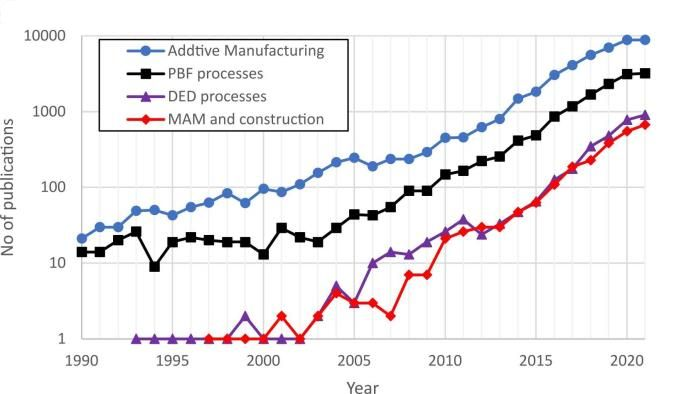
\includegraphics[width=1\textwidth]{search5}
	\ccaption{Anzahl an wissenschaftlichen Artikeln und Publikationen zum Thema 3D-Druck}{adaptierte Grafik, von \protect\cite{KANYILMAZ2022102541} entnommen}
	\label{img:search_5}
\end{figure}
Wie aus Abb. \ref{img:search_5} erkennbar ist, ist die Nachfrage und Forschung für die Anwendung des 3D-Drucks, besonders für die \acrlong{slm}- und \acrfull{pbf}-Prozesse, stark angestiegen in den letzten beiden Jahrzehnten.

\begin{figure}[H]
	\centering
	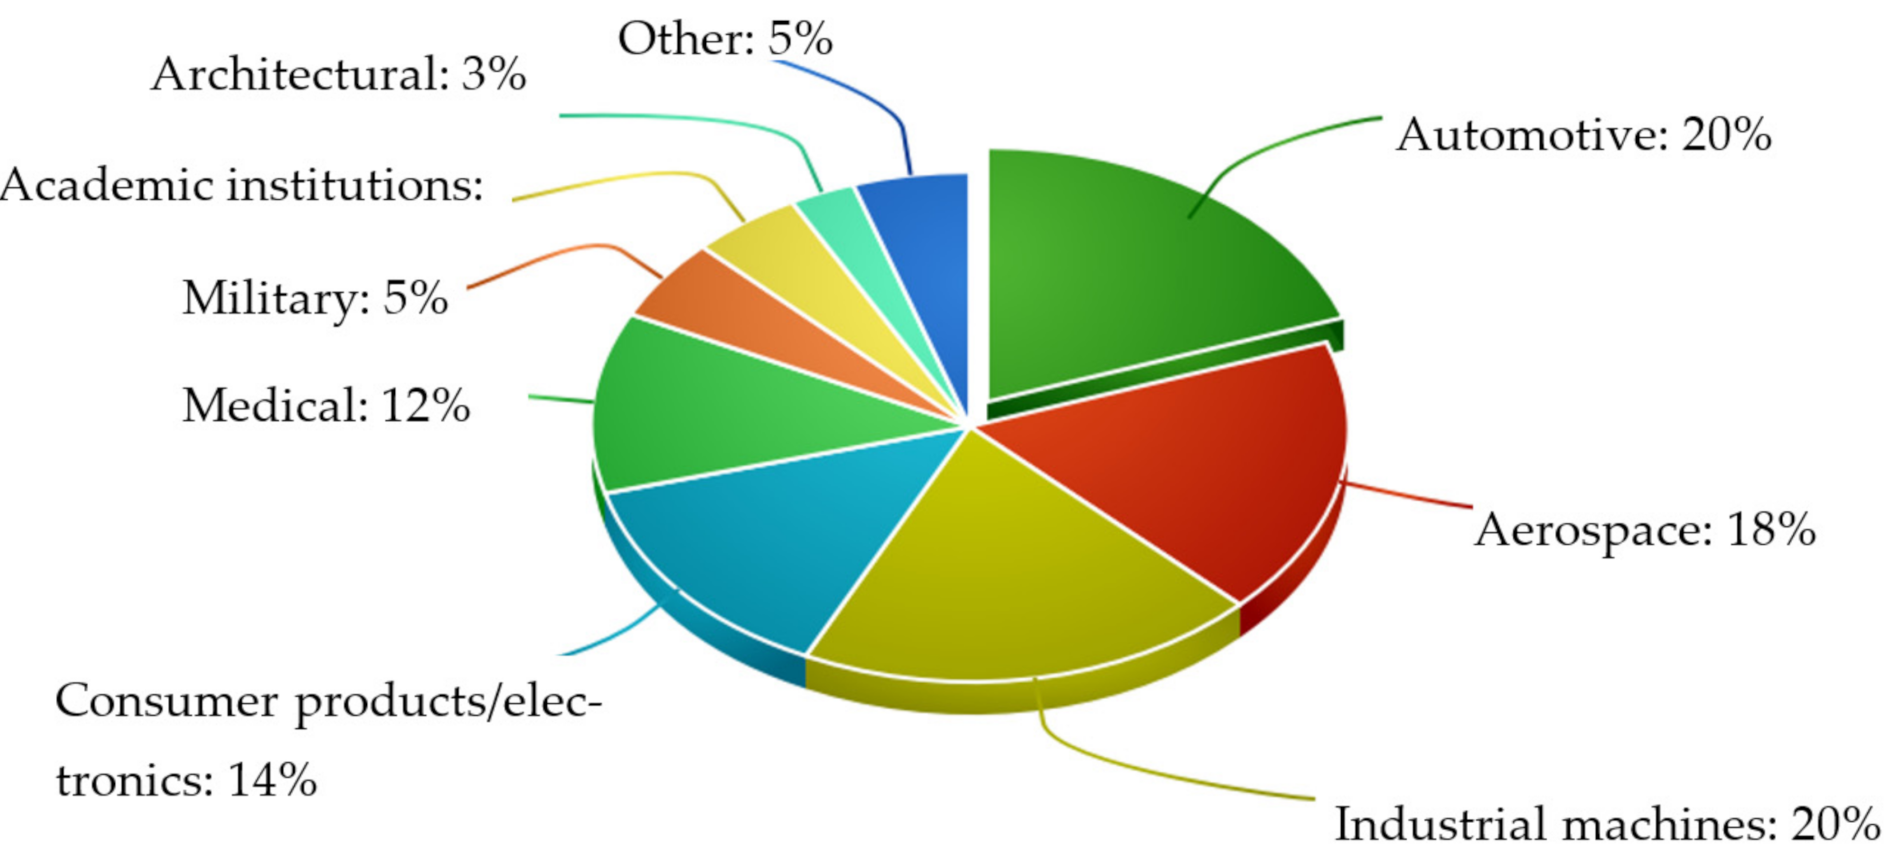
\includegraphics[width=1\textwidth]{am_shares}
	\ccaption{Anteile verschiedener Anwendungsgebiete im \acrshort{am} (Stand 2017) }{Grafik von \protect\cite{app11031213} entnommen}
	\label{img:am_shares}
\end{figure} 
\subsection{Forschung}
\subsubsection{Medizinische Implantate}
\paragraph{Zahntechnische Anwendungen}
Abb. \ref{img:dental} beschreibt den Aufbau eines 3D-gedruckten Zahn-Implantates 
\begin{figure}[H]
	\centering
	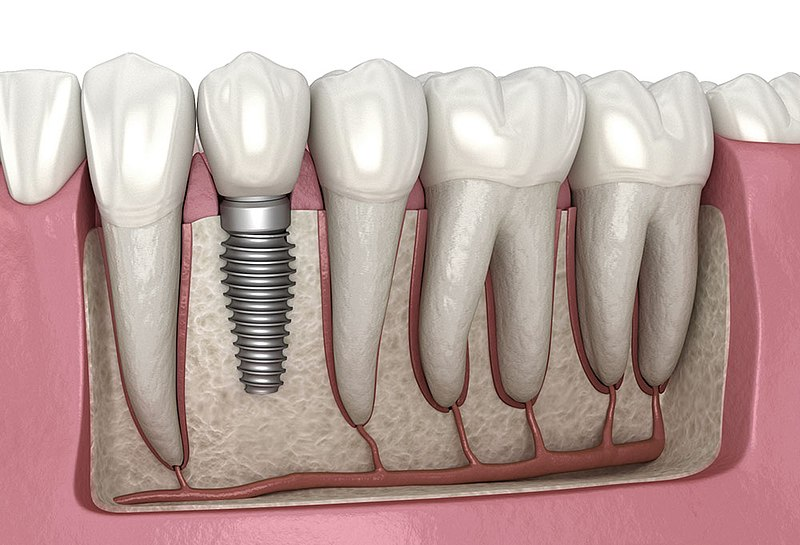
\includegraphics[width=.6\textwidth]{dental}
	\ccaption{Grafische Darstellung eines Zahnimplantates mit 3D-gedruckter Zahn-Krone}{https://upload.wikimedia.org/wikipedia/commons/1/1d/Dental-implant-illustration.jpg}
	\label{img:dental}
\end{figure} 
 
\subsection{Industrie}
\subsubsection{Reparatur und OOP-Ersatzteil-Produktion}
Das durchschittliche Alter industriell verwendeter Maschinen liegt bei 15+ Jahren \parencite{lifespan_1}, wobei die meisten dieser Maschinen sowie auch ihre Ersatzteile bereits \acrfull{oop} sind. 
Restbestände sind nur mehr für sehr hohe Preise verfügbar und mit logistischem Aufwand verbunden. 
Oft ist es dadurch effizienter für Firmen neue Maschinen anzuschaffen, obwohl die existierenden Geräte bis auf einzelne Bauteile noch gut funktionieren. 
Auch logistische Probleme sind ein großer hindernder Faktor für den Zugriff auf Ersatzteile, besonders in Bereichen wie Schiffsfahrt oder Luftfahrt. Der Transport eines Schiffspropellers, welche zumeist mehrere Tonnen wiegen, ist logistisch sehr kompliziert und teuer.  
Mithilfe eines LMD-ähnlichen Prozesses ist es aber möglich besagten Teil lokal zu produzieren \parencite{ship_1} und dabei Transport- und Lagerkosten sowie auch viel Zeit zu sparen. 

Bei dem obigen Beispiel wird der Teil komplett neu produziert. 
Eine für viele Industrien realistischere Option ist die Reparatur eines beschädigten Teils. Für eine komplette Reproduktion wäre ein \acrshort{cad}-Modell nötig, um die nötige Präzision zu erhalten. 
Bei einer teilweisen Rekonstruktion kann mithilfe von speziellen Messgeräten und Scannern die Impräzision des \acrshort{lmd}-Prozesses minimiert werden und im Nachhinein noch mit Substratktiven Verfahren wie \acrfull{cnc} oder Drehen auf die genaue Spezifikation angepasst werden. 
\subsubsection{Leichtbauindustrie}

\subsubsection{Automobil-Industrie}

\end{document}
